\documentclass[11pt,a4paper]{article}
\usepackage[utf8]{inputenc}
\usepackage[T1]{fontenc}
\usepackage[british]{babel}
\usepackage{lmodern,microtype,amsmath,amssymb}
\usepackage[margin=24mm]{geometry}
\usepackage{booktabs,tabularx,array,longtable}
\usepackage{tikz,pgfplots}
\pgfplotsset{compat=1.17}
\usepackage{xcolor,float}
\usepackage[colorlinks=true,linkcolor=blue!45!black,citecolor=blue!45!black,urlcolor=blue!45!black]{hyperref}
\usepackage{bookmark}
\newcommand{\code}[1]{\texttt{\detokenize{#1}}}
\newcommand{\norm}[1]{\left\lVert#1\right\rVert}
\newcommand{\R}{\mathbb{R}}
\newcommand{\dt}{\Delta t}
\newcommand{\repo}{\url{https://github.com/javoxa/YoguiCuentas}}
\newcommand{\autores}{Javier Armando Gutierrez}
\newcommand{\afiliacion}{Departamento de Física, FCE, Universidad Nacional de Salta\\\small Salta, Argentina\\\small\href{mailto:g.javier.ar@gmail.com}{g.javier.ar@gmail.com}}
\setlength{\parskip}{3pt}
\emergencystretch=3em
\hypersetup{pdftitle={Implementation of an educational heat-conduction simulator with low computational cost},pdfauthor={Javier Armando Gutierrez},pdfsubject={Technical report for peer review, British English translation, 6 November 2026}}
\title{Implementation of an educational heat-conduction simulator with low computational cost\\[2mm]\large Coarse grids and OpenGL visualisation}
\author{\autores\\[2mm]\small\afiliacion}
\date{6 November 2026\\\small British English translation of Spanish revision 2 (2 November 2026)\\\small Verification campaigns: 28--29 October 2026}
\begin{document}
\maketitle
\begin{abstract}
YoguiCuentas is a two-dimensional educational heat-conduction simulator intended for resource-constrained computers. Its design separates the grid on which the heat equation is solved from image resolution: OpenGL turns a field with relatively few nodes into maps and animated surfaces, without requiring one thermal unknown per pixel. The number of nodes can therefore be chosen to meet the physical requirements of an exercise, whilst rendering provides its visual presentation. Computation can run on the CPU whilst retaining the available graphics acceleration for visualisation, an option relevant to laboratories without dedicated GPUs. Field transfer, interpolation and publication of committed states are described alongside a conservative model incorporating materials, sources and boundary conditions. Euler, Crank--Nicolson, Jacobi and Gauss--Seidel methods support investigations of evolution and refinement cost. NumPy/OpenCL and Swift/Metal verification campaigns assess balances and analytical references; the recorded timings characterise the solver rather than the OpenGL frame rate. Conditions under which a coarse grid is sufficient are discussed: visual continuity neither adds physical resolution nor corrects geometric errors. The contribution is a practical educational tool combining accessible hardware requirements, interactive visualisation and a verifiable physical basis.
\end{abstract}
\noindent\textbf{Keywords:} educational simulation; heat conduction; limited resources; OpenGL rendering; coarse grids; scientific visualisation.




\section{Introduction}
Heat-transfer work in a teaching laboratory requires a tool with which a problem can be constructed, its conditions changed and the response observed. Exploring a different material, a localised source or a convective boundary is particularly useful when the response can be viewed during the activity. In this setting, the value of simulation includes ease of use and the availability of suitable computers, as well as numerical accuracy.

A high-resolution image does not require a thermal grid with an equal number of points. For smooth problems, the field can be represented by a moderate number of nodes and subsequently drawn over many more pixels. Refining the equation solely to obtain a visually continuous image incurs avoidable cost: it increases the number of unknowns and, with an explicit integrator, reduces the permitted time step. The design problem is to resolve the physics on a grid appropriate to the exercise and use the graphics system to produce its visual representation.

YoguiCuentas \cite{yogui} is being developed for this purpose. Its Linux edition combines a CPU or OpenCL solver with OpenGL rendering; users can edit geometries, assign materials, sources and boundary conditions, and inspect temperature and heat-flux fields. Visualisation remains available when thermal computation runs on the CPU. The macOS edition adapts the environment to Swift/Metal and provides another implementation against which numerical results can be compared. This article focuses on the application of rendering to an educational tool with modest hardware requirements; verification provides the physical basis for the displayed behaviour.

The separation of numerical and screen resolution is described, identifying which operations remain proportional to the number of nodes and what a coarse grid can achieve. The thermal model, methods and verification experiments are then documented. Teaching applications, hardware accessibility and the limitations of the approach are discussed. Numerical verification is distinguished from validation against physical measurements \cite{nasa-verify,nasa-grid}; the latter is outside the available campaigns.

\section{Design for resource-constrained computers}
\subsection{Solving few nodes and drawing many pixels}
The numerical field contains $N=n_xn_y$ temperatures. The image occupies $P=W\,H$ pixels, where $W$ and $H$ are the drawing-area dimensions. These quantities are independent: enlarging the window changes rasterisation without creating new thermal unknowns. For a complete rectangular domain, the drawing mesh uses the existing nodes and $2(n_x-1)(n_y-1)$ triangles. OpenGL interpolates vertex values when generating fragments and applies the colour map through shaders \cite{glsl}.

For example, a $33\times33$ grid contains 1089 temperatures and produces 2048 triangles in the rectangular case. It can be displayed over $1280\times720$ pixels without solving 921600 thermal equations. This is an illustrative size comparison, not a speed measurement. Graphics work still depends on the pixels, layers and device, but does not entail an equal number of heat-equation evaluations.

On each planar triangle, the visual reconstruction is
\begin{equation}
 \widetilde T(\mathbf x)=\lambda_1(\mathbf x)T_1+\lambda_2(\mathbf x)T_2+\lambda_3(\mathbf x)T_3,\qquad \sum_{a=1}^{3}\lambda_a=1.
 \label{eq:render}
\end{equation}
The weights describe triangle interpolation, not a new solution of the problem. In a rectangle, reconstruction is piecewise linear over triangles; it is not claimed to be exactly bilinear throughout each cell. For cut-outs, the code constructs fans over active dual volumes and combines only locally connected nodes, avoiding primitives that cross excluded regions. The 3D surface raises this mesh according to temperature; a small number of vertices retains a faceted geometry even when the colour appears continuous.

\begin{figure}[tbp]\centering
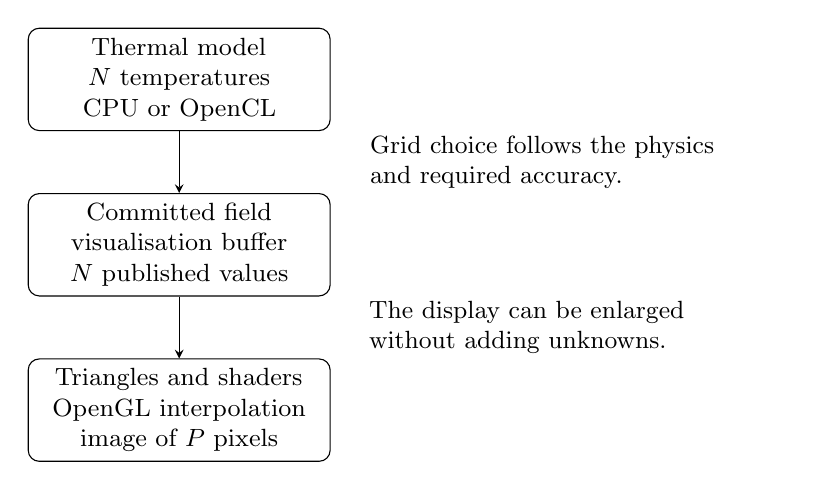
\begin{tikzpicture}[every node/.style={font=\small,align=center},>=stealth]
\node[draw,rounded corners,text width=3.6cm,minimum height=1.3cm] (a) at (0,0) {Thermal model\\$N$ temperatures\\CPU or OpenCL};
\node[draw,rounded corners,text width=3.6cm,minimum height=1.3cm] (b) at (0,-2.1) {Committed field\\visualisation buffer\\$N$ published values};
\node[draw,rounded corners,text width=3.6cm,minimum height=1.3cm] (c) at (0,-4.2) {Triangles and shaders\\OpenGL interpolation\\image of $P$ pixels};
\draw[->] (a)--(b);
\draw[->] (b)--(c);
\node[anchor=west,align=left,text width=5.3cm] at (2.3,-1.05) {Grid choice follows the physics\\and required accuracy.};
\node[anchor=west,align=left,text width=5.3cm] at (2.3,-3.15) {The display can be enlarged\\without adding unknowns.};
\end{tikzpicture}
\caption{Separation of computation and presentation on Linux. This implementation diagram is neither a benchmark nor a screenshot. The CPU path retains OpenGL rendering; when supported, the shared OpenCL/OpenGL path avoids routing the field through the host.}\label{fig:pipeline}
\end{figure}

\subsection{Computation, transfer and animation}
In the CPU path, NumPy updates the thermal field in a worker and publishes a float32 snapshot to an OpenGL buffer. This path requires compatible graphics hardware for drawing, but no dedicated GPU for thermal computation. When OpenCL and OpenGL share a context, the application copies the computed field to a shared VBO without first reading it into host memory. A publication copy remains: sharing resources does not remove every copy or synchronisation operation.

Buffer ownership is ordered through a sequence of graphics waiting, OpenCL acquisition, copying, release and drawing. A host-transfer path is available when interoperability is unsupported. Each image corresponds to a committed state; the editor, solver and visible image are not conflated into a single mutable field. This design allows the latest available solution to remain on screen without requiring a physical step to coincide with each displayed frame.

In the CPU path, publication is limited to approximately 30 updates per second. This scheduling limit avoids unnecessary transfers; it is neither a measured nor a guaranteed frame rate. Several simulation steps may occur between publications, or a step may take longer than that interval. Users can pause, change playback speed and inspect the state without interpreting screen time as physical time.

\subsection{What low cost means in this work}
The objective is to reduce the resources required for a particular activity: unknown count, computational storage, work per step and reliance on a dedicated accelerator. A single float32 field with $33^2$ nodes occupies 4356 bytes; one with $257^2$ nodes occupies 264196 bytes, approximately 60.65 times as much. The programme maintains other buffers and uses interface and graphics memory, so these figures are not its total RAM consumption.

The main saving comes from avoiding grid refinement solely for presentation. Once physical resolution has been chosen, rendering uses the available graphics hardware for maps, surfaces and indicators. The approach supports integrated graphics when the driver supplies the required functions; CPU computation does not remove the Linux interface's OpenGL requirement. The current edition uses GLSL 1.40 and texture buffers, so compatibility must be checked on each computer.

As preliminary evidence of feasibility, installation and CPU use were reported on laboratory computers with Intel i3-3240/i5-4440 processors and 4/8 GB RAM. These practical trials motivate the design; instrumented frame-rate, peak-memory and latency records are not available for those models. The formal campaigns below use Ryzen/A2000 and M1 systems. Reported usability is therefore distinguished from quantitative characterisation of the laboratory hardware, which remains outstanding.

A coarse grid is appropriate when it resolves the spatial scales relevant to the exercise. It may show diffusion of a smooth profile or heat-exchange trends without matching screen resolution in the solver. A narrow source, poorly represented interface or steep gradient requires refinement and verification. Continuous colour assists interpretation; it neither creates physical information between nodes nor turns an inadequate approximation into an accurate solution.

\section{Physical model and discretisation}
\subsection{Continuous problem and units}
For a planar domain $\Omega$, consider
\begin{equation}
 C(\mathbf{x})\frac{\partial T}{\partial t}=\nabla\!\cdot(k(\mathbf{x})\nabla T)+Q(\mathbf{x}),\qquad C=\rho c_p>0,\quad k>0.
 \label{eq:pde}
\end{equation}
Here $T$ is temperature; $k$ is conductivity in W\,m$^{-1}$\,K$^{-1}$; $C$ is volumetric heat capacity in J\,m$^{-3}$\,K$^{-1}$; and $Q$ is volumetric heat generation in W\,m$^{-3}$. Properties are temperature-independent within the tested scope. The two-dimensional representation integrates balances per unit thickness: energy is expressed in J/m and power in W/m. Temperature differences are expressed in K although the interface displays temperatures in degrees Celsius.

The boundary may prescribe temperature $T=T_b$, outward heat flux $-k\nabla T\cdot\mathbf n=q_N$, or convection $-k\nabla T\cdot\mathbf n=h_b(T-T_\infty)$, with $h_b\geq0$. The adiabatic case has zero flux. Radiation, advection, phase change and temperature-dependent properties are excluded; their validity is not inferred from these results.

\subsection{Grid, dual volumes and operator}
The nodal Cartesian grid is uniform along each axis, with $\Delta x=L_x/(n_x-1)$ and $\Delta y=L_y/(n_y-1)$, which may differ. Each active node has a dual volume $V_i$ per unit thickness. Outer volumes of the rectangular box have reduced widths, and masks determine the participating connections and exposed faces. No boundary-fitted mesh is generated from the drawn curves.

For the unconstrained degrees of freedom, the balance is
\begin{equation}
 C_iV_i\dot T_i=\sum_{j\in\mathcal N(i)}G_{ij}(T_j-T_i)+Q_iV_i-\sum_{b\in\mathcal B(i)}P_{ib},\qquad G_{ij}=\frac{k_{ij}a_{ij}}{d_{ij}}.
 \label{eq:balance}
\end{equation}
Here $a_{ij}$ is face length per unit thickness and $d_{ij}$ is the node separation. Face conductivity follows from resistances in series; equal half-distances give $k_{ij}=2k_ik_j/(k_i+k_j)$. Symmetric conductance allows internal exchanges to cancel in the total balance. Prescribed-temperature nodes are not free unknowns; their thermal reactions must be considered when interpreting global energy.

At an internal cut-out, the wall lies half a cell away. The Robin condition combines conductive and convective resistance:
\begin{equation}
 G_{ib}^{R}=\frac{a_{ib}}{d_{ib}/k_i+1/h_b},\qquad d_{ib}\in\{\Delta x/2,\Delta y/2\}.
 \label{eq:robin}
\end{equation}
This distance must not be indiscriminately assigned to the outer nodes of the box: the implementation distinguishes the two representations. A cut-out Dirichlet temperature is imposed through conductance to its face, whereas the box fixes its outer nodes. Corners with two prescribed temperatures retain the implemented averaging convention.

Assembly gives
\begin{equation}
 \dot{\mathbf T}=\mathbf f-A\mathbf T,\qquad r(\mathbf T)=\mathbf f-A\mathbf T,
 \label{eq:ode}
\end{equation}
with residual $r_i$ in K/s. The stencil has five points; boundary losses contribute to the diagonal and forcing. Steady-state solution requires a thermal reference in each connected free component. Purely Neumann/adiabatic components are rejected by the current steady-state mode: a general null-space treatment with a mean constraint has not been implemented.

Version 2 scenes represent area sources with $8\times8$ subcell sampling and line sources with power per unit length. This quadrature is a rasterisation choice, not an exact geometric reconstruction. Adjacent active regions retain conduction between materials; exclusion creates exposed faces to which boundary conditions are assigned.

\section{Methods and solution checks}
\subsection{Time integration and steady-state solution}
Explicit Euler uses $\mathbf T^{n+1}=\mathbf T^n+\dt\,r(\mathbf T^n)$. For the diffusive structure with non-negative coefficients, the step is limited using the loss diagonal and a safety factor. For a homogeneous rectangle without additional losses, this recovers $\alpha\dt(\Delta x^{-2}+\Delta y^{-2})\leq1/2$, where $\alpha=k/C$. Increasing the node count reduces the permissible step.

Crank--Nicolson (CN) \cite{crank} solves
\begin{equation}
 (I+\dt A/2)\mathbf T^{n+1}=(I-\dt A/2)\mathbf T^n+\dt\mathbf f.
\end{equation}
The implementation uses increments $\delta=\mathbf T^{n+1}-\mathbf T^n$:
\begin{equation}
 (I+\theta\dt A)\delta=\dt\,r(\mathbf T^n),
 \label{eq:increment}
\end{equation}
with $\theta=1/2$ for CN. Weighted Jacobi with $\omega=2/3$ solves the system, and the increment-system residual is checked in K. Selecting Gauss--Seidel for steady state does not replace this internal solver. If a system fails to converge, the batch is rejected; a partial field is not published as a solution.

Optional Rannacher start-up replaces the first physical step by two backward-Euler steps of length $\dt/2$, with $\theta=1$, before continuing with CN. It damps high-frequency components in irregular data \cite{rannacher}. For $\dot u=-\lambda u$ and $z=\lambda\dt$,
\begin{equation}
 g_E=1-z,\qquad g_{CN}=\frac{1-z/2}{1+z/2},\qquad g_R=(1+z/2)^{-2}.
 \label{eq:gains}
\end{equation}
CN stability guarantees neither positivity nor absence of sign changes: at $z=4$, $g_{CN}=-1/3$, whereas start-up gives $g_R=1/9$.

For steady state, $A\mathbf T=\mathbf f$, weighted Jacobi and red--black Gauss--Seidel (GS), with $\omega=1$ for GS, are available. Jacobi updates simultaneously from the previous field. GS colours nodes by index parity and updates red then black through ordered dispatches; a complete iteration includes both colours. This ordering produces different iterates from lexicographic GS. Both methods are iterative \cite{templates}; the Spanish interface label ``estacionario directo'' denotes absence of time integration, not direct factorisation. Their CSV files count iterations without assigning physical time to them.

\subsection{Physical residual and educational stopping criteria}
The default criterion simultaneously requires
\begin{align}
 R_\infty&=\max_{i\in F}|r_i|\leq a_r+\varepsilon_rR_\infty^{(0)},\\
 B_1&=\sum_{i\in F}C_iV_i|r_i|\leq a_r\sum_{i\in F}C_iV_i+\varepsilon_rB_1^{(0)},
 \label{eq:residual}
\end{align}
where $F$ contains active free nodes. $B_1$ has units W/m and sums local absolute values; it is not a signed net balance that could vanish through cancellation. General defaults are $a_r=10^{-5}$ K/s and $\varepsilon_r=10^{-5}$, checked every 128 steps with three consecutive confirmations. Tests may override these values and record them; the defaults are not universal accuracy tolerances.

Change-based criteria use $D=T^{(c)}-T^{(c-1)}$ between committed fields at consecutive checks. When checking every $N$ steps, $D$ spans those $N$ steps, not a graphics frame or half a GS sweep. The first check compares against the initial condition. Table~\ref{tab:criteria} defines the nine options. For matrix measures, $D=0$ outside the selection.

\begin{table}[tbp]\centering\small
\caption{Available criteria. $S$ is the node selection and $m=|S|$; indices $i,j$ in the two matrix measures denote row and column.}\label{tab:criteria}
\begin{tabularx}{\linewidth}{@{}lX@{}}\toprule
Criterion & Measure or condition\\\midrule
Physical residual & Equations~\eqref{eq:residual}, always at all free nodes.\\
$\Delta T$ L1 & $\sum_S|D_i|$.\\
Euclidean/Frobenius & $\sqrt{\sum_SD_i^2}$.\\
RMS & $\sqrt{\sum_SD_i^2/m}$.\\
Nodal maximum & $\max_S|D_i|$, equal to the vector infinity norm.\\
Matrix 1-norm & $\max_j\sum_i|D_{ij}|$.\\
Matrix infinity norm & $\max_i\sum_j|D_{ij}|$, distinct from the nodal maximum.\\
Trace/diagonal sum & $|\sum_iD_{ii}|$ over the eligible diagonal.\\
Change in mean & $|\sum_SD_i/m|$.\\\bottomrule
\end{tabularx}
\end{table}

The eight $\Delta T$ measures are compared with $a_\Delta+\varepsilon_\Delta s$, in K, with scale $s$ computed from $T-T_{ref}$. For the trace and mean, scaling uses absolute values rather than a signed sum. Vector and matrix norms are distinguished according to their definitions \cite{numpy-norm}. The trace and change in mean are not norms: opposing changes may cancel. The trace ignores off-diagonal variation and is termed the diagonal sum on a rectangular grid. A diagonal with no free nodes cannot confirm the criterion.

All of $F$, or a fixed sample drawn without replacement, may be observed. A partial Fisher--Yates permutation using a 32-bit congruential generator and a recorded seed reproduces the selection across implementations; it is not redrawn at each check. Sampling may miss relevant regions and provides no coverage guarantee. The full physical audit remains active even with sampling. Sampling therefore supports comparison and does not remove the cost of auditing the full domain.

The selected criterion and the audit have independent counters. Outcomes distinguish \code{converged} (both confirmed), \code{criterion_met} (change criterion satisfied without confirmed physical equilibrium) and \code{max_steps} (budget exhausted). A tiny time step can produce small $D\simeq\dt r$ whilst $r$ remains large. This separation avoids automatically equating apparent immobility with steady state. None of these conditions alone bounds temperature error against the continuous problem.

\section{Implementation and traceability}
The Linux edition uses Python, NumPy, PyOpenCL and a Tkinter/OpenGL interface; the macOS edition uses SwiftUI, AppKit and Metal, with SceneKit surface rendering. NumPy computes in float64; OpenCL, Swift CPU and Metal GPU use float32 fields. Metal host-side checks accumulate in Double, which cannot recover precision lost when updating the float32 field.

JSON v1/v2 scenes preserve geometry and assignments. Computation produces a committed field separate from editor requests and the field awaiting publication. Changing processor resets and pauses the run. Captures and isotherms correspond to the published field; isotherm levels are equally spaced in temperature, not necessarily in spatial distance. One level may produce several connected curves. The 3D representation is a surface of the two-dimensional field, not a three-dimensional conduction solution.

Exports store the CSV field, scenario, metadata and a history of up to 512 checks, with truncation indicated. Metadata identify requested and effective processor, steps or iterations, tolerances, residuals and stopping reason. OpenCL retains the previous check field on the GPU and reads 15 scalars per check; this transfer path is not attributed to the Metal solver. Conceptually matching formats do not imply binary identity or identical arithmetic operations.

The analysed campaigns concern developments after Linux 0.2.4 and Metal 0.11.0, in a working tree modified relative to its base commit. The distribution candidate is identified as Linux 0.2.5 and Metal 0.12.0. These later version numbers must not be confused with accepted executions of final installers. Packaging metadata changes made after testing are distinguished from the numerical sources tested.

\section{Materials and verification methodology}
\subsection{Hardware and precision}
The Linux campaign ran on an AMD Ryzen 9 5900X, Linux 6.12.95, Python 3.11.2 and NumPy 1.26.4, using an NVIDIA RTX A2000 as local OpenCL device 1. Recorded versions were NVIDIA driver 570.86.10, OpenCL 3.0 CUDA and PyOpenCL 2026.1.2. The index identifies that inventory and must be queried again on another machine.

The macOS campaign used an Apple M1 with a seven-core GPU and 8 GiB unified memory, macOS 15.4.1 (24E263), Xcode 16.4 and Swift 6.1.2. M1 measurements were made on battery at a recorded charge of 74\%, without workload isolation or power measurement. These conditions limit performance analysis and do not support conclusions about energy efficiency. Version numbers describe campaign records, not minimum software requirements.

\subsection{References and error separation}
Analytical references, semi-discrete solutions and balances independent of the stopping criterion were used. For a homogeneous rectangular sinusoidal mode,
\begin{equation}
 u(x,y,t)=\sin(\pi x/L_x)\sin(\pi y/L_y)e^{-\lambda t},\qquad
 \lambda=\alpha\big[(\pi/L_x)^2+(\pi/L_y)^2\big].
\end{equation}
the corresponding discrete eigenvalue is
\begin{equation}
 \lambda_h=4\alpha\left[\frac{\sin^2(\pi\Delta x/(2L_x))}{\Delta x^2}+\frac{\sin^2(\pi\Delta y/(2L_y))}{\Delta y^2}\right].
\end{equation}
These tests use $k=1$ W/(m K), $C=10$ J/(m$^3$ K), initial amplitude 1 K and homogeneous Dirichlet boundaries. These are verification parameters, without fitting to a physical experiment. Temporal refinement is compared with $e^{-\lambda_ht}$ to separate spatial and temporal errors. Steps $\dt=0.04,0.02,0.01$ s are used up to $t=0.4$ s on a $9\times7$ grid. Spatial refinement uses the continuous solution on $17\times9$, $33\times17$ and $65\times33$ grids up to $t=0.02$ s; Euler reduces $\dt$ approximately as $h^2$ and CN uses $\dt=0.002$ s. Observed orders are calculated as
\begin{equation}
 p=\frac{\log(e_h/e_{h/2})}{\log2},\qquad e=\norm{T_{num}-T_{ref}}_\infty.
 \label{eq:order}
\end{equation}
These are three-level studies of smooth cases. Neither a Grid Convergence Index (GCI) nor general uncertainty for arbitrary scenarios is calculated; the observed order does not automatically extend to cut-out geometries \cite{nasa-grid}.

Steady-state tests include a source-driven parabolic profile, a two-material interface with resistances in series, and a linear profile with Neumann/Robin boundaries. The interface is positioned halfway between nodes to isolate the operator from interface displacement. A circle with a uniform source and Dirichlet boundary is compared with $T(r)=T_b+Q(R^2-r^2)/(4k)$. Conservation is tested in rectangular and elliptical domains, with heterogeneity and sources. In isolated systems, discrete energy $E=\sum_iC_iV_iT_i$ must change according to source input; with Neumann/Robin conditions, outward flux is integrated. Euler uses initial flux and CN its temporal average, consistently with their discretisations.

\subsection{Specified tolerances}
On Linux, CN systems use $a_{CN}=10^{-13}$ K and $\varepsilon_{CN}=10^{-12}$ for NumPy, and $10^{-8}$ K and $10^{-6}$ for OpenCL. Steady-state profiles use absolute residual tolerances of $10^{-10}$ K/s and $2\times10^{-5}$ K/s, respectively, with zero relative tolerance. Temperature error ($2\times10^{-8}$ K and $2\times10^{-4}$ K) and interface flux ($10^{-7}$ and $5\times10^{-4}$ W/m$^2$) are also checked. These thresholds belong to those tests; they are neither physical constants nor guaranteed programme accuracy.

The supplementary M1 circular-refinement test specifies a residual tolerance of $10^{-4}$ K/s; it does not replace the original $33^2$-node test at $5\times10^{-5}$ K/s. Specific limits and complete parameters remain in JSON files, logs and test sources. A residual target of $10^{-10}$ K/s is also imposed in float32 to verify that stagnation is reported as non-convergence. Thresholds are not silently relaxed to convert a limit exit into success.

\subsection{Computational-cost protocol}
The M1 benchmark comprises $5\times4\times2\times3=120$ measurements: sizes $17^2$, $33^2$, $65^2$, $129^2$ and $257^2$; four methods; two processors; and three repetitions. Compilation uses \code{-O}; four steps/sweeps provide warm-up and 64 are timed. Cost scenarios use a unit box, $k=1$, $C=10$, sinusoidal amplitude 1 K and zero boundary temperature; Euler uses $0.8\,\dt_{lim}$ and CN $8\,\dt_{lim}$. Initialisation and kernel compilation are excluded; Metal includes dispatch, field upload and read-back, and CN includes all internal iterations. The interface, CSV writing and steady-state audits external to the CN solver are excluded. Medians are reported per combination; three repetitions alone do not characterise a statistical performance distribution.

Comparisons use the same fixed count within each method, not equal physical time between integrators or equal final error between methods. A GS sweep includes both colours. The Linux benchmark uses a different transfer path; its data are retained but are not used as a controlled A2000--M1 comparison.

\section{Results}
\subsection{Tests, conservation and observed orders}
Table~\ref{tab:counts} separates suites and experiments to avoid adding checks of different kinds. The two Linux skips concern native mouse clicks with a locked desktop, not skipped GPU numerical tests. All 103 M1 XCTest cases passed without failures or skips. The subsequent Linux review recalculated integrity and metrics from the received evidence; it neither ran Metal on Linux nor constituted independent reproduction on a second M1.

\begin{table}[tbp]\centering\small
\caption{Campaign evidence. Rows overlap and must not be added as independent sample sizes.}\label{tab:counts}
\begin{tabularx}{\linewidth}{@{}lX@{}}\toprule
Record & Result or contents\\\midrule
Linux suite, 29 October & 155 passed, 2 skipped; 157 discovered, no failures.\\
Linux physical campaign & 217 checks passed.\\
Linux criterion comparison & 64 comparative cases, including equilibrium errors.\\
Final M1 suite & 103 XCTest cases passed; no failures or skips.\\
M1 numerical data & 60 NUMERIC records.\\
Supplementary M1 campaign & 158 records: 144 criteria, 6 circles, 4 modal factors and 4 balances.\\
M1 exports & 144 audited field/scenario/metadata/history sets.\\
M1 cost & 120 timings; 8 field pairs saved for comparison.\\\bottomrule
\end{tabularx}
\end{table}

The maximum absolute error in the four independent M1 transient Neumann/Robin balances was $7.88148\times10^{-8}$ J/m, against a $2\times10^{-6}$ J/m limit. Cancellation of internal exchanges and consistent integration of sources and boundaries were also checked in the Linux campaign. Conservation is a property of the discrete problem tested; it does not guarantee that the represented boundary matches the intended physical geometry.

% BEGIN AUTO ORDER_TABLE
\begin{table}[tbp]\centering\small
\caption{Observed orders across three refinement levels. Each cell gives the two successive orders.}\label{tab:orders}
\begin{tabular}{@{}lrrrr@{}}\toprule
Implementation & Temporal Euler & Temporal CN & Spatial Euler & Spatial CN\\\midrule
NumPy & 1.0275 / 1.0135 & 2.0008 / 2.0002 & 2.0095 / 1.9996 & 1.9966 / 2.0042\\
OpenCL & 1.0275 / 1.0135 & 2.0011 / 2.0159 & 2.0112 / 2.0730 & 1.9970 / 2.0026\\
Swift & 1.0275 / 1.0135 & 2.0011 / 2.0159 & 2.0047 / 1.9456 & 1.9953 / 1.9795\\
Metal & 1.0275 / 1.0135 & 2.0011 / 2.0159 & 2.0065 / 1.9410 & 1.9953 / 1.9820\\
\bottomrule\end{tabular}\end{table}
% END AUTO ORDER_TABLE

The orders in Table~\ref{tab:orders} are consistent with first-order Euler and second-order CN over the range studied. Spatial orders near two concern the smooth rectangular case. Figure~\ref{fig:temporal} shows the original error magnitudes as well as supporting the calculated orders. Float32 deviations are expected as truncation error decreases and rounding becomes significant.

% BEGIN AUTO TEMPORAL_FIGURE
\begin{figure}[tbp]\centering
\begin{minipage}{.49\linewidth}\centering
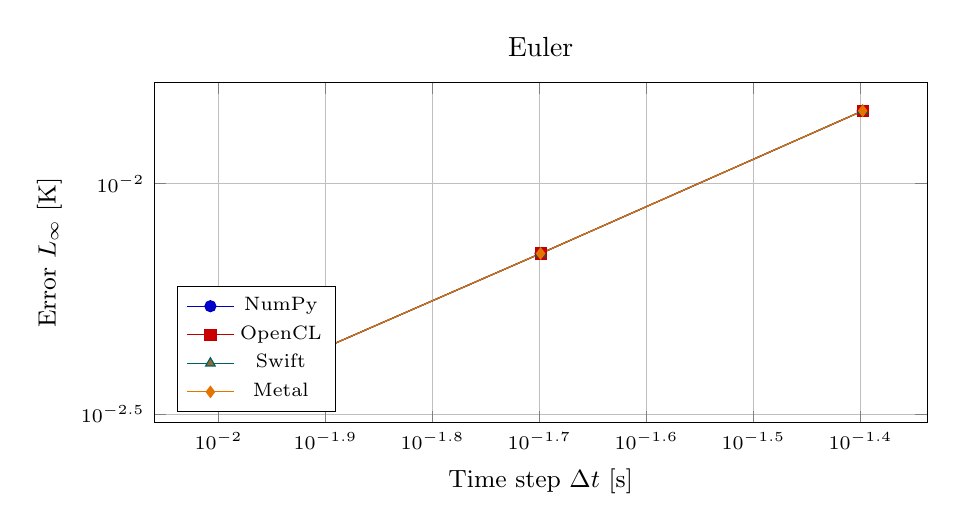
\begin{tikzpicture}
\begin{loglogaxis}[width=.94\linewidth,height=5.9cm,title={Euler},xlabel={Time step $\Delta t$ [s]},ylabel={Error $L_\infty$ [K]},grid=major,legend style={font=\scriptsize,at={(0.03,0.03)},anchor=south west},tick label style={font=\scriptsize},label style={font=\small},scaled ticks=false]
\addplot+[color=blue!75!black,mark=*,solid] coordinates {(0.04,0.0143793971491) (0.02,0.00705392559814) (0.01,0.00349415537512)};
\addlegendentry{NumPy}
\addplot+[color=red!75!black,mark=square*,solid] coordinates {(0.04,0.0143793874969) (0.02,0.00705391704935) (0.01,0.00349414884943)};
\addlegendentry{OpenCL}
\addplot+[color=teal!75!black,mark=triangle*,solid] coordinates {(0.04,0.0143793278922) (0.02,0.00705373823541) (0.01,0.00349397003549)};
\addlegendentry{Swift}
\addplot+[color=orange!90!black,mark=diamond*,solid] coordinates {(0.04,0.0143792384853) (0.02,0.00705373823541) (0.01,0.00349397003549)};
\addlegendentry{Metal}
\end{loglogaxis}\end{tikzpicture}\end{minipage}
\begin{minipage}{.49\linewidth}\centering
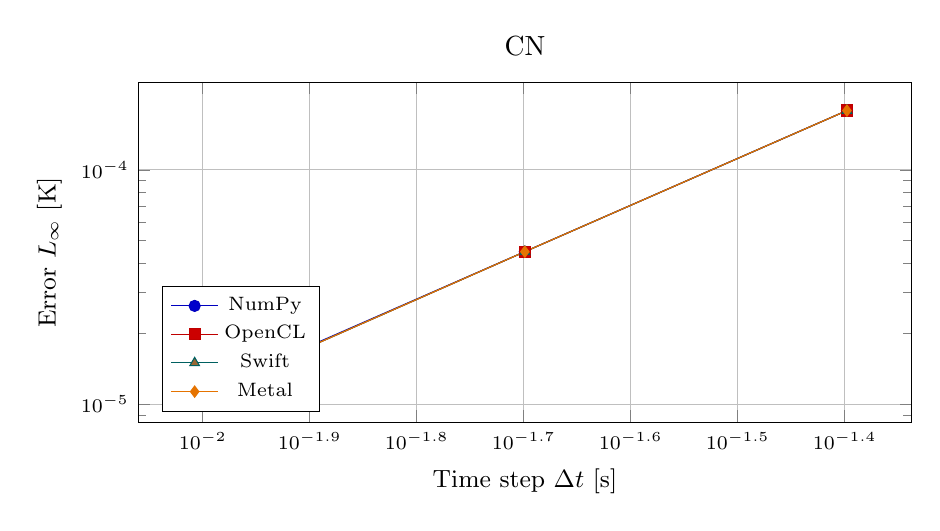
\begin{tikzpicture}
\begin{loglogaxis}[width=.94\linewidth,height=5.9cm,title={CN},xlabel={Time step $\Delta t$ [s]},ylabel={Error $L_\infty$ [K]},grid=major,legend style={font=\scriptsize,at={(0.03,0.03)},anchor=south west},tick label style={font=\scriptsize},label style={font=\small},scaled ticks=false]
\addplot+[color=blue!75!black,mark=*,solid] coordinates {(0.04,0.000179135052711) (0.02,4.47599751149e-05) (0.01,1.11885085458e-05)};
\addlegendentry{NumPy}
\addplot+[color=red!75!black,mark=square*,solid] coordinates {(0.04,0.000179087518632) (0.02,4.47386493085e-05) (0.01,1.10620250104e-05)};
\addlegendentry{OpenCL}
\addplot+[color=teal!75!black,mark=triangle*,solid] coordinates {(0.04,0.000179087518632) (0.02,4.47386493085e-05) (0.01,1.10620250104e-05)};
\addlegendentry{Swift}
\addplot+[color=orange!90!black,mark=diamond*,solid] coordinates {(0.04,0.000179087518632) (0.02,4.47386493085e-05) (0.01,1.10620250104e-05)};
\addlegendentry{Metal}
\end{loglogaxis}\end{tikzpicture}\end{minipage}
\caption{Temporal refinement against the semi-discrete mode, $9\times7$ nodes, $t=0.4$ s. CPU/GPU curves nearly overlap; they are not eight independent replicates. Points are recorded errors, without fitting.}\label{fig:temporal}
\end{figure}
% END AUTO TEMPORAL_FIGURE

For the high-frequency mode $z=4$, Swift gave $g_{CN}=-0.333333254$ and Metal $-0.333333373$; both recorded $g_R=0.111111104$. Agreement with Equation~\eqref{eq:gains} shows that CN oscillations may arise from the method rather than a drawing error. Initial damping does not justify arbitrarily large steps without assessing temporal accuracy.

\subsection{Stopping, sampling and export consistency}
The 144 M1 cases combine four methods, two processors, two node selections and nine criteria. They produced 72 \code{converged} and 72 \code{max_steps} outcomes. The deliberately short budget was 64 steps; the latter are neither 72 failed tests nor evidence of divergence. The suite verifies that stopping reasons reflect counters and budgets. Separate tiny-step tests require \code{criterion_met} when variation settles before the physical residual.

The audit of all 144 export sets checked field dimensions, coordinates, finite temperatures, requested/effective processor, final step and history, and consistency with the scenario. Steady-state methods do not assign physical seconds to iterations. This evidence supports export contracts for the tested cases, not exhaustive validation of every possible scene or user action.

\subsection{Accuracy across implementations}
Across the 120 M1 measurements, the maximum recorded Swift/Metal difference at equal counts was $1.54972\times10^{-6}$ K. Reconstruction in float32 from eight saved CSV pairs, covering four methods and sizes $17^2$ and $65^2$, gave a maximum of $1.49012\times10^{-6}$ K. These are different sets, so their maxima need not coincide. Bitwise equality is not claimed.

Forty-eight Linux/M1 pairs of errors against analytical references were compared. This compares errors rather than A2000 and M1 fields directly. Nor does it establish complete independence: the implementations share the formulation, scenarios and part of the test design. OpenCL showed stagnation of some profiles near $10^{-6}$ K/s; a mixed-boundary GS case settled around $2.27\times10^{-6}$ K/s. A tolerance incompatible with float32 does not improve the field and should produce an informative outcome.

\subsection{Circular geometry and Robin bias}
For $R=0.31$ m, $k=1$ W/(m K), $Q=4$ W/m$^3$ and $T_b=0$, maximum Metal errors for the Dirichlet circle were $0.0129054$, $0.00603398$ and $0.00269434$ K at $17^2$, $33^2$ and $65^2$ nodes. Refinement improves this case without establishing a universal order for curved domains.

The circular Robin test reveals a more persistent limitation (Table~\ref{tab:robin}). The circle is centred in a $0.5\times0.5$ m box, with radius $R=0.2$ m, $h_b=15$ W/(m$^2$ K) and $k=401$ W/(m K). Discrete convective conductance at the stair-stepped boundary is measured and compared with $h_b2\pi R$ per unit thickness. Units are W/(m K); for a thickness of 1 m, the numerical value equals the conductance in W/K. This comparison characterises boundary representation, rather than the total radial resistance between centre and surroundings.

% BEGIN AUTO ROBIN_TABLE
\begin{table}[tbp]\centering\small
\caption{Circular Robin conductance per unit thickness, in W/(m K). The source field labels unit-thickness conductance as W/K.}\label{tab:robin}
\begin{tabular}{@{}lrrr@{}}\toprule
Grid & $G_h$ & $G_{ideal}$ & Excess [\%]\\\midrule
$41^2$ & 24.744215 & 18.849556 & 31.272\\
$81^2$ & 24.372151 & 18.849556 & 29.298\\
$161^2$ & 24.186086 & 18.849556 & 28.311\\
\bottomrule\end{tabular}\end{table}
% END AUTO ROBIN_TABLE

The axis-aligned-face approximation measures a Manhattan-type length. For a circle of radius $R$, the limiting sum of horizontal and vertical projections is $8R$, compared with $2\pi R$. As half-cell resistance tends to zero under refinement, Equation~\eqref{eq:robin} retains the geometric factor
\begin{equation}
 \frac{8R}{2\pi R}-1=\frac4\pi-1\simeq27.32395\%.
 \label{eq:bias}
\end{equation}
The observed 28.31\% error at $161^2$ nodes is consistent with this limit; three grids do not establish a general numerical proof for every mask sequence. The geometric argument explains why additional nodes cannot remove the bias. The corresponding test passes by detecting this limitation, not by certifying accuracy for the ideal circle. Resolution requires appropriate boundary metrics, not merely tighter solver tolerances.

% BEGIN AUTO ROBIN_FIGURE
\begin{figure}[tbp]\centering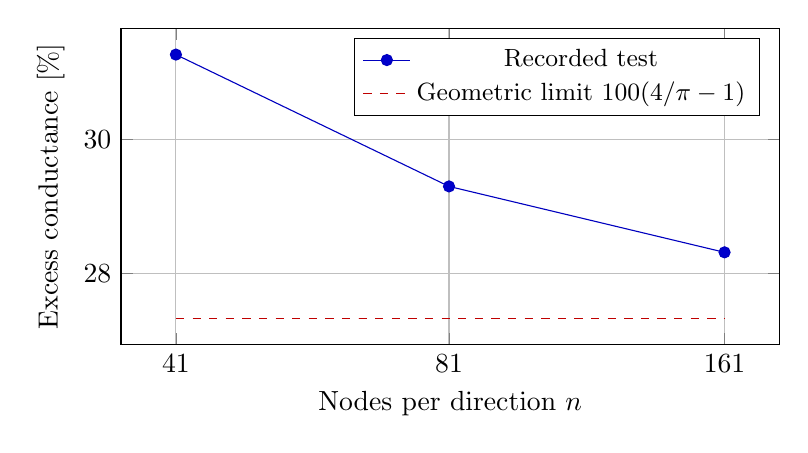
\begin{tikzpicture}
\begin{axis}[width=.82\linewidth,height=5.6cm,xmode=log,log basis x=2,xlabel={Nodes per direction $n$},ylabel={Excess conductance [\%]},grid=major,xtick={41,81,161},xticklabels={41,81,161},legend style={font=\small,at={(0.97,0.97)},anchor=north east}]
\addplot+[blue!75!black,mark=*,solid] coordinates {(41,31.272137869) (81,29.2982769062) (161,28.3111733837)};
\addlegendentry{Recorded test}
\addplot[red!75!black,dashed,domain=41:161] {27.3239544735};
\addlegendentry{Geometric limit $100(4/\pi-1)$}
\end{axis}\end{tikzpicture}
\caption{Refinement reduces part of the boundary error but not the limiting excess stair-stepped perimeter. The horizontal line is the geometric prediction, not a fit to the three points.}\label{fig:robin}\end{figure}
% END AUTO ROBIN_FIGURE

\subsection{Cost and problem size}
% BEGIN AUTO TIMING_TABLE
\begin{table}[tbp]\centering\small
\caption{Median time for 64 steps/sweeps at $257^2$ nodes, three repetitions. The ratio compares processors within each method, not efficiency between methods.}\label{tab:timing}
\begin{tabular}{@{}lrrr@{}}\toprule
Method & Swift [s] & Metal [s] & Swift/Metal\\\midrule
Euler & 0.016355 & 0.002231 & 7.33\\
CN & 1.793044 & 0.350358 & 5.12\\
Jacobi & 0.035471 & 0.002535 & 13.99\\
GS & 0.041021 & 0.005071 & 8.09\\
\bottomrule\end{tabular}\end{table}
% END AUTO TIMING_TABLE

At $257^2$ nodes, median Swift/Metal time ratios were 7.33 (Euler), 5.12 (CN), 13.99 (Jacobi) and 8.09 (GS). Swift is faster in some small cases (Figure~\ref{fig:cost}). Dispatch, synchronisation and data movement can dominate when each batch contains little work. CN includes many internal sweeps and must not be compared with one Euler step as though both had equal cost or accuracy.

% BEGIN AUTO COST_FIGURE
\begin{figure}[tbp]\centering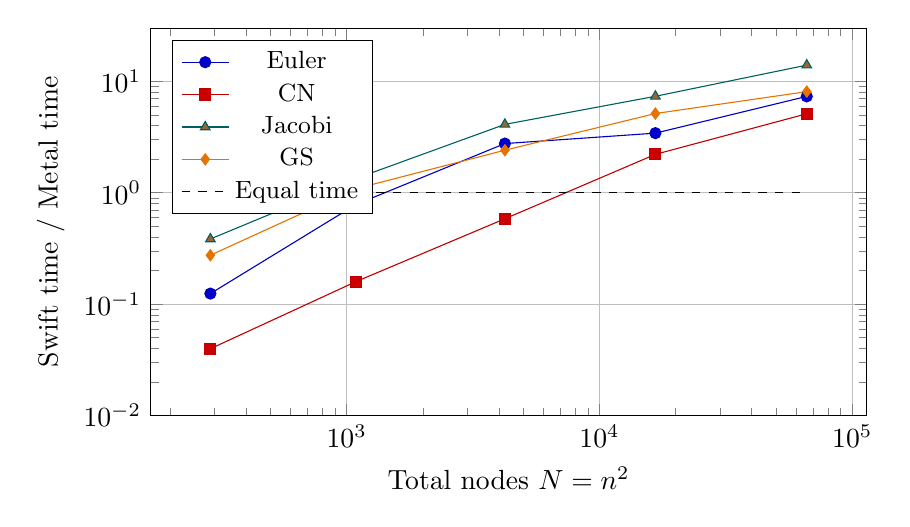
\begin{tikzpicture}
\begin{loglogaxis}[width=.88\linewidth,height=6.5cm,xlabel={Total nodes $N=n^2$},ylabel={Swift time / Metal time},grid=major,legend style={font=\small,at={(0.03,0.97)},anchor=north west},ymin=0.01,ymax=30]
\addplot+[color=blue!75!black,mark=*,solid] coordinates {(289,0.124326917455) (1089,0.784185541088) (4225,2.76435931438) (16641,3.4285364775) (66049,7.33132856925)};
\addlegendentry{Euler}
\addplot+[color=red!75!black,mark=square*,solid] coordinates {(289,0.0397652082676) (1089,0.159357607202) (4225,0.583819500579) (16641,2.21176556916) (66049,5.11774617299)};
\addlegendentry{CN}
\addplot+[color=teal!75!black,mark=triangle*,solid] coordinates {(289,0.384366173701) (1089,1.34248106992) (4225,4.10932622676) (16641,7.34436903152) (66049,13.9904680555)};
\addlegendentry{Jacobi}
\addplot+[color=orange!90!black,mark=diamond*,solid] coordinates {(289,0.274799409118) (1089,1.08838227425) (4225,2.41004319184) (16641,5.14271829338) (66049,8.08897380011)};
\addlegendentry{GS}
\addplot[black,dashed,domain=289:66049] {1};\addlegendentry{Equal time}
\end{loglogaxis}\end{tikzpicture}
\caption{Ratios of M1 median times for 64 steps/sweeps. Values above one favour Metal; values below one favour Swift. Metal field transfers are included; time to equal error is not measured and A2000 is not compared with M1.}\label{fig:cost}\end{figure}
% END AUTO COST_FIGURE

Each stencil application requires work and storage proportional to node count $N$ for a fixed number of buffers. For a fixed-size physical region in 2D with an approximately isotropic grid, $N=O(h^{-2})$; the explicit limit $\dt=O(h^2)$ gives $O(h^{-4})=O(N^2)$ operations to reach a fixed physical time when each application has linear cost. This is an asymptotic argument, not a fit to campaign timings. Steady-state sweep counts depend on convergence; CN also depends on its internal solver. Neither peak memory nor electrical energy was measured here, so practical bounds for all computers cannot be given.

\section{Discussion: a practical tool for the teaching laboratory}
The educational purpose is to let a student construct a case, change a condition and observe its evolution without relying on a high-performance computer. Rendering has a specific role: it makes a field with relatively few nodes readable, allows switching between maps, surfaces and heat flux, and retains animation when computation runs on the CPU. Continuous visualisation helps users follow moving hot regions and approach to equilibrium, whilst the nodes remain the unknowns of a defined thermal model.

This separation gives the teacher two distinct choices. A coarse grid can be retained to explore trends, with refinement reserved for an accuracy comparison. The drawing area can also be enlarged or the camera changed without modifying the numerical problem. Improving presentation therefore need not increase solver cost. This benefit is particularly relevant to laboratories using repurposed computers without a dedicated GPU at every workstation.

The tool retains energy balances, heterogeneous conductivity, sources and thermal boundary conditions alongside transient and steady-state methods. This basis supports activities beyond illustrative animation. An initial exercise may examine a smooth profile on a coarse grid, export temperatures and compare with a reference solution. Repeating the exercise with more nodes reveals changes in both field and cost. Screen interpolation keeps both cases readable; numerical comparison determines whether the initial grid was sufficient.

Another exercise changes a source, material or boundary and uses heat-flux and isotherm overlays to interpret thermal exchange. Isotherm levels are equally spaced in temperature, not distance: clustering may indicate steep gradients. The 3D surface helps interpret the two-dimensional field, but its height and relief are visual devices. They represent neither three-dimensional conduction nor measured physical height.

Stopping controls prevent an apparently motionless animation from being mistaken for equilibrium. A point sample, trace or mean may settle whilst local changes persist. The residual audit makes that difference inspectable within the same environment. Similarly, the high-frequency CN test explains method-related sign changes, and circular refinement exposes a geometric error that rendering cannot correct.

Available data support the tested computations and show that CPU computation may be advantageous for small problems. Accessibility on modest computers is supported by the architecture and reported practical trials, but quantification requires a dedicated interactive-performance campaign. Timings for 64 steps cannot establish the frame rate of a window displaying isotherms and a 3D surface. Student learning outcomes were not measured either: the activities described are proposed applications whose educational value requires evaluation in context.

\section{Limitations and future development}
Low-cost examples require a grid adequate for the observed phenomenon. In particular, a small node count does not ensure accurate representation of narrow sources or curved boundaries. The current implementation uses structured Cartesian grids. Curves and materials are rasterised; the circular Robin bias is an explicit limitation. Unstructured meshes, fitted curvilinear boundaries, radiation and temperature-dependent properties are unavailable. Unreferenced steady-state components require future null-space treatment. Iterative solution and float32 arithmetic limit attainable tolerances.

A proposed next stage is planar-polar discretisation for circular geometries, including treatment of the origin, angular periodicity, consistent areas and normals, and new conservation and order tests. A polar grid may remain structured; it must not automatically be described as unstructured. Unstructured meshes for general geometries form a separate development direction. The Robin result requires geometric metrics to be verified before improvements are inferred from node count.

The numerical campaigns did not complete manual acceptance of the M1 editor/interface, first launch on another Mac, Gatekeeper behaviour, or final Debian/Devuan installation and removal. The received app has a local ad hoc signature, without Developer ID or notarisation. Two Linux native-click tests remain skipped because the session was locked. These tasks affect distribution acceptance, although they do not in themselves invalidate the documented numerical measurements. A fully verified production distribution is not claimed.

\section{Conclusions}
An educational environment separating heat-equation resolution from image resolution has been implemented. OpenGL displays a field computed with relatively few nodes as maps and animated surfaces; window size does not force an increase in unknown count. This application of rendering directs numerical work towards the physics required by the exercise and retains a CPU computation path for computers without a dedicated compute GPU.

The tool integrates scenario editing, materials, sources, boundaries, transient and steady-state methods, and result export. Verification supports interpreting its images as representations of a conservative model within the studied cases and tolerances. Visual smoothness remains distinct from accuracy: refinement is needed when the problem demands it, and Robin bias at a stair-stepped circular boundary requires correcting geometry rather than drawing.

Low cost is framed as an implementation choice and the use of coarse grids, supported by reported operation on modest laboratory computers. Characterising it as a hardware performance claim requires frame-rate, latency and memory measurements on those computers with specified scenes and accuracy. The current outcome is an open tool for exploring thermal phenomena with limited resources, accompanied by numerical evidence through which its scope can be assessed and further improvements developed.

\section*{Code, data availability and reproducibility}
The project repository is \repo. Project code and documentation are distributed under Apache License 2.0 within the scope stated in \code{LICENSE} and \code{NOTICE}; this work does not extend rights over images or third-party material. Bibliographic sources retain their respective rights.

The analysed evidence is identified by the manifests and paths in the appendix. The local candidate and this manuscript do not yet constitute a deposited publication with a DOI; public availability of the specific revision must be checked at submission. The base commit of a modified working tree does not by itself identify every tested file. An archival version should deposit sources, data, manifests and this manuscript together under a persistent identifier, without retrospectively attributing a non-existent DOI.

\section*{Authorship, funding and declarations}
Corresponding author: Javier Armando Gutierrez, Departamento de Física, FCE, Universidad Nacional de Salta, Salta, Argentina; \href{mailto:g.javier.ar@gmail.com}{g.javier.ar@gmail.com}. The corresponding author is responsible for final review and submission. No funding or competing-interest statement has been supplied; this absence is not replaced by a declaration that none exists. This manuscript was prepared with assistance from an artificial-intelligence tool for artefact inspection, organisation, drafting and figure generation from recorded data. Human authors must review and take responsibility for the content, results and disclosure required by the publication venue. The tool is not assigned authorship.

\appendix
\section{Evidence identification and reproduction}
The Linux campaign of 29 October records a working tree modified relative to base commit
\begin{quote}\small\ttfamily\raggedright
\detokenize{58742d505561a9e75466dca0ec0f748e0b285dc0}.
\end{quote}
The combined hash of numerical sources is
\begin{quote}\small\ttfamily\raggedright
\detokenize{e576c94fc46a53d1efabf29c9b291d2569dd7580370554cb8f50788dda384c78}.
\end{quote}
The M1 return was checked against 71/71 final files, 32/32 test-manifest entries, 18/18 benchmark entries and 1374/1374 delivery files. The public selection retains 635 files with its own manifest. The received binary matches
\begin{quote}\small\ttfamily\raggedright
\detokenize{22ae2a2609a65878a755ebc0b64570f4e3b8c9c6581096444e6af9b2e2d9237d}.
\end{quote}
Signing is evidenced by the received macOS log; Linux verified the hash without rerunning \code{codesign}. Subsequently, only the Metal packaging script's default version was changed to 0.12.0; the integrated Swift computational sources and tests retained their tested bytes at the time of the Spanish revision. The later interface-localisation changes are outside these campaigns and require separate acceptance. Documentary traceability does not amount to rerunning the installer.

\begin{table}[htbp]\centering\footnotesize
\caption{Locations of principal artefacts relative to the repository root.}\label{tab:artifacts}
\begin{tabularx}{\linewidth}{@{}lX@{}}\toprule
Artefact & Path\\\midrule
Linux metadata and metrics & \path{verification/2026-10-29/numerical/report.json}\\
Full Linux suite & \path{verification/2026-10-29/unittest.log}\\
Linux criteria & \path{verification/2026-10-29/criteria/README.md}\\
Final M1 suite & \path{verification/2026-10-29/m1/final-02/swift-test.log}\\
M1 measurements and scenarios & \path{verification/2026-10-29/m1/final-02/}\\
M1 cost & \path{verification/2026-10-29/m1/benchmark-final/timings.csv}\\
Return audit & \path{verification/2026-10-29/m1-review/audit.json}\\
M1 evidence manifest & \path{verification/2026-10-29/m1/MANIFIESTO_EVIDENCIA.sha256}\\
Table/figure data & \path{technical_report/datos_manuscrito.json}\\\bottomrule
\end{tabularx}
\end{table}

To run the Linux campaign without the graphical interface:
\begin{quote}\small\ttfamily\raggedright
python -m yoguicuentas.verification --backend numpy\par
\hspace*{1em}--skip-benchmark --output resultados/verificacion\par
python -m yoguicuentas.verification --backend opencl --device INDEX\par
\hspace*{1em}--skip-benchmark --output resultados/verificacion-gpu
\end{quote}
Each command spans two typographical lines and must be executed as one line. Obtain the device index using \code{python -m yoguicuentas --list-devices}. Requesting OpenCL without an available device must fail explicitly. For the complete M1 campaign, from the repository root:
\begin{quote}\small\ttfamily\raggedright
bash metal/yoguicuentas\_metal/verificar\_numerica.sh\par
\hspace*{1em}verification/repeticion full
\end{quote}
The preceding command must also be joined onto one line. Execution requires Swift tools and a Metal-capable Mac to avoid skipping GPU tests; a downloaded app does not include the XCTest environment. Logs must retain failures and skips. The script \code{technical_report/preparar_datos.py} regenerates the Spanish manuscript's data and figure segments; numbers come from the identified records, without synthetic data. The English LaTeX file is self-contained, including bibliography and plot coordinates. Its translated captions must be retained when updating generated data.

\section{Complete M1 cost summary}
% BEGIN AUTO FULL_TIMING_TABLE
\begin{table}[H]\centering\small
\caption{Medians of the 120 M1 timings, grouped into 40 size/method/processor combinations. Scenarios and individual repetitions are retained with the evidence.}\label{tab:full-cost}
\begin{tabular}{@{}rlrrr@{}}\toprule
$n_x=n_y$ & Method & Swift [s] & Metal [s] & Swift/Metal\\\midrule
17 & Euler & 0.0000654 & 0.0005262 & 0.124\\
17 & CN & 0.0074421 & 0.1871517 & 0.040\\
17 & Jacobi & 0.0002719 & 0.0007073 & 0.384\\
17 & GS & 0.0003767 & 0.0013710 & 0.275\\
33 & Euler & 0.0006045 & 0.0007709 & 0.784\\
33 & CN & 0.0368816 & 0.2314394 & 0.159\\
33 & Jacobi & 0.0013004 & 0.0009687 & 1.342\\
33 & GS & 0.0016968 & 0.0015590 & 1.088\\
65 & Euler & 0.0023663 & 0.0008560 & 2.764\\
65 & CN & 0.1347383 & 0.2307876 & 0.584\\
65 & Jacobi & 0.0031762 & 0.0007729 & 4.109\\
65 & GS & 0.0030916 & 0.0012828 & 2.410\\
129 & Euler & 0.0040920 & 0.0011935 & 3.429\\
129 & CN & 0.5324523 & 0.2407363 & 2.212\\
129 & Jacobi & 0.0072743 & 0.0009905 & 7.344\\
129 & GS & 0.0097022 & 0.0018866 & 5.143\\
257 & Euler & 0.0163547 & 0.0022308 & 7.331\\
257 & CN & 1.7930442 & 0.3503582 & 5.118\\
257 & Jacobi & 0.0354705 & 0.0025353 & 13.990\\
257 & GS & 0.0410212 & 0.0050712 & 8.089\\
\bottomrule\end{tabular}\end{table}
% END AUTO FULL_TIMING_TABLE

\clearpage
\begin{thebibliography}{9}
\bibitem{glsl} J. Kessenich / The Khronos Group. \emph{The OpenGL Shading Language}, version 1.40, revision 08, 22 November 2009. Official specification; input/output and interpolation sections. \url{https://registry.khronos.org/OpenGL/specs/gl/GLSLangSpec.1.40.pdf}. Accessed 2 November 2026.
\bibitem{crank} J. Crank and P. Nicolson. A practical method for numerical evaluation of solutions of partial differential equations of the heat-conduction type. \emph{Proceedings of the Cambridge Philosophical Society}, 43(1), 50--67, 1947. \href{https://doi.org/10.1017/S0305004100023197}{doi:10.1017/S0305004100023197}. Reprinted in: \emph{Advances in Computational Mathematics}, 6, 207--226, 1996, \href{https://doi.org/10.1007/BF02127704}{doi:10.1007/BF02127704}.
\bibitem{rannacher} R. Rannacher. Finite element solution of diffusion problems with irregular data. \emph{Numerische Mathematik}, 43, 309--327, 1984. \href{https://doi.org/10.1007/BF01390130}{doi:10.1007/BF01390130}.
\bibitem{templates} R. Barrett, M. Berry, T. F. Chan, J. Demmel, J. M. Donato, J. Dongarra, V. Eijkhout, R. Pozo, C. Romine and H. van der Vorst. \emph{Templates for the Solution of Linear Systems: Building Blocks for Iterative Methods}. SIAM, 1994. \url{https://netlib.org/templates/templates.html}.
\bibitem{nasa-verify} NPARC Alliance / NASA Glenn Research Center. \emph{Verification Assessment}. Verification and validation tutorial. \url{https://www.grc.nasa.gov/www/wind/valid/tutorial/verassess.html}. Accessed 30 October 2026.
\bibitem{nasa-grid} NPARC Alliance / NASA Glenn Research Center. \emph{Examining Spatial (Grid) Convergence}. Verification and validation tutorial. \url{https://www.grc.nasa.gov/www/wind/valid/tutorial/spatconv.html}. Accessed 30 October 2026.
\bibitem{numpy-norm} NumPy Developers. \emph{numpy.linalg.norm}: vector and matrix norms. Official documentation. \url{https://numpy.org/doc/stable/reference/generated/numpy.linalg.norm.html}. Accessed 30 October 2026.
\bibitem{yogui} YoguiCuentas Project. \emph{YoguiCuentas sources, scenarios and numerical evidence}. Campaigns of 28--29 October 2026, developments after Linux 0.2.4 and Metal 0.11.0. \repo. Revision identified by the appendix manifests; no DOI assigned in this manuscript.
\end{thebibliography}
\end{document}
